\documentclass[11pt]{beamer}
% \usetheme{Boadilla}
  \usetheme{default}


% acronyms for text or math mode
\newcommand {\ccast} {\mbox{\small CCAST}}
\newcommand {\cris} {\mbox{\small CrIS}}

\newcommand {\airs} {\mbox{\small AIRS}}
\newcommand {\iasi} {\mbox{\small IASI}}
\newcommand {\idps} {\mbox{\small IDPS}}
\newcommand {\nasa} {\mbox{\small NASA}}
\newcommand {\noaa} {\mbox{\small NOAA}}
\newcommand {\nstar} {\mbox{\small STAR}}
\newcommand {\umbc} {\mbox{\small UMBC}}
\newcommand {\uw}   {\mbox{\small UW}}

\newcommand {\fft}  {\mbox{\small FFT}}
\newcommand {\ifft} {\mbox{\small IFFT}}
\newcommand {\fir}  {\mbox{\small FIR}}
\newcommand {\fov}  {\mbox{\small FOV}}
\newcommand {\for}  {\mbox{\small FOR}}
\newcommand {\ict}  {\mbox{\small ICT}}
\newcommand {\ils}  {\mbox{\small ILS}}
\newcommand {\igm}  {\mbox{\small IGM}}
\newcommand {\opd}  {\mbox{\small OPD}}
\newcommand {\rms}  {\mbox{\small RMS}}
\newcommand {\zpd}  {\mbox{\small ZPD}}
\newcommand {\ppm}  {\mbox{\small PPM}}
\newcommand {\srf}  {\mbox{\small SRF}}
\newcommand {\sdr}  {\mbox{\small SDR}}

\newcommand {\ES} {\mbox{\small ES}}
\newcommand {\SP} {\mbox{\small SP}}
\newcommand {\IT} {\mbox{\small IT}}
\newcommand {\SA} {\mbox{\small SA}}

\newcommand {\ET} {\mbox{\small ET}}
\newcommand {\FT} {\mbox{\small FT}}

% abbreviations, mainly for math mode
\newcommand {\real} {\mbox{real}}
\newcommand {\imag} {\mbox{imag}}
\newcommand {\atan} {\mbox{atan}}
\newcommand {\obs}  {\mbox{obs}}
\newcommand {\calc} {\mbox{calc}}
\newcommand {\sinc} {\mbox{sinc}}
\newcommand {\psinc} {\mbox{psinc}}
\newcommand {\std} {\mbox{std}}

% symbols, for math mode only
\newcommand {\wnum} {\mbox{cm$^{-1}$}}
\newcommand {\lmax} {L_{\mbox{\tiny max}}}
\newcommand {\vmax} {V_{\mbox{\tiny max}}}

\newcommand {\tauobs} {\tau_{\mbox{\tiny obs}}}
\newcommand {\taucal} {\tau_{\mbox{\tiny calc}}}
\newcommand {\Vdc}  {V_{\mbox{\tiny DC}}}

\newcommand {\rIT} {r_{\mbox{\tiny\textsc{ict}}}}
\newcommand {\rES} {r_{\mbox{\tiny\textsc{es}}}}
\newcommand {\robs} {r_{\mbox{\tiny obs}}}

\newcommand {\rITobs} {r_{\mbox{\tiny\textsc{ict}}}^{\mbox{\tiny obs}}}
\newcommand {\rITcal} {r_{\mbox{\tiny\textsc{ict}}}^{\mbox{\tiny cal}}}

\newcommand {\ITmean} {\langle\mbox{\small IT}\rangle}
\newcommand {\SPmean} {\langle\mbox{\small SP}\rangle}


\title{apodization of CrIS \\ 
       extended interferograms
}
\author{H.~E.~Motteler and L.~L.~Strow}
\institute{
UMBC Atmospheric Spectroscopy Lab \\
  Joint Center for Earth Systems Technology \\
}
\date{\today}
\begin{document}

%----------- slide --------------------------------------------------%
\begin{frame}[plain]
\titlepage
\end{frame}
%----------- slide --------------------------------------------------%
\begin{frame}
\frametitle{introduction}

\begin{itemize}

  \item we show that applying a cosine apodization at the edges of
    the new extended interferograms reduces sweep direction and
    {\fov} 5 relative residuals, in comparison to processing without
    such apodization

  \item results are from a three day test period, 8-10 Nov 2015

  \item all test are done with the {\ccast} reference calibration
    algorithm, processing filters as presented in our 5 May 2015
    telecon talk, periodic sinc wrapping at the sensor grid, and
    double Fourier interpolation to the user grid

  \item tests with the {\noaa} reference calibration algorithm would
    be significant, but were not done in time for this presentation
    
\end{itemize}

\end{frame}
%----------- slide --------------------------------------------------%
\begin{frame}
\frametitle{CrIS resolution modes}

\begin{itemize}

  \item \umbc\ \ccast\ sensor-grid resolution modes include

\begin{tabular}{crrrl}
   mode  &  LW  &   MW  &  SW  &  comment  \\
   \hline
  lowres &  866 &   530 &  202 &  low res  \\
  hires1 &  866 &  1039 &  799 &  old high res  \\
  hires2 &  866 &  1052 &  799 &  2014 high res  \\
  hi3to2 &  866 &  1052 &  800 &  truncation test  \\
  hires3 &  874 &  1052 &  808 &  new extended res  \\
\end{tabular}

  \item {\ccast} user-grid resolution modes include the original
    0.8/0.4/0.2 {\wnum} {\opd} low res mode and the 0.8 {\wnum}
    {\opd} high res mode

  \item double Fourier interpolation from the sensor to user grid
    allows for any combination of sensor and user resolutions

  \item interferogram centers are at decimated points $n/2 + 1$
    for even point sets.  The center is at $n/2 + 1$ for the 799
    point set as well, but in that case is not an integer

\end{itemize}

\end{frame}
%----------- slide --------------------------------------------------%
\begin{frame}
\frametitle{interferogram centers}
\begin{center}
  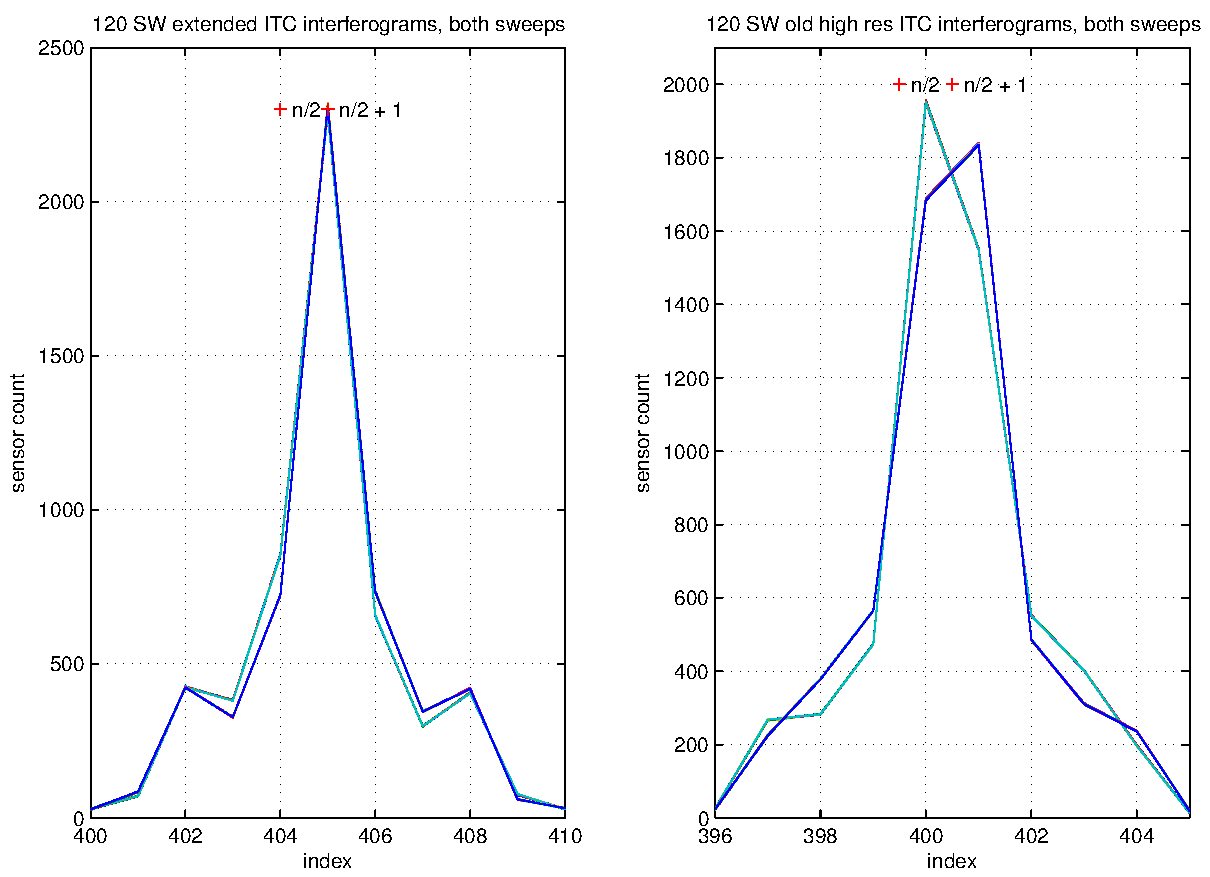
\includegraphics[scale=0.4]{figures/igm_SW_centers.pdf}
\end{center}
center detail of phase-corrected interferograms for 120 SW ICT
looks (one 60-scan granule), including both sweep directions
\end{frame}
%----------- slide --------------------------------------------------%
\begin{frame}
\frametitle{extended interferogram apodization}

\begin{itemize}
  \item we can drop 6 points on each side of the extended resolution
    interferograms and stay very close to the {\opd} spec

 \item $(n - 12) \cdot dx =$ 1.5995 for the LW, 1.6081 for the MW,
   and 1.6001 for the SW bands, for typical metrology laser values

 \item this includes the MW band, even though that was not extended
   in the recent update

 \item apodizing (rather than dropping) these points leaves
   effective resolution within specs

 \item note that the apodized extension discussed here is distinct
   from any downstream apodization (such as Hamming) that is applied
   to user-grid radiances

\end{itemize}

\end{frame}
%----------- slide --------------------------------------------------%
\begin{frame}
\frametitle{extended interferogram apodization}
\begin{center}
  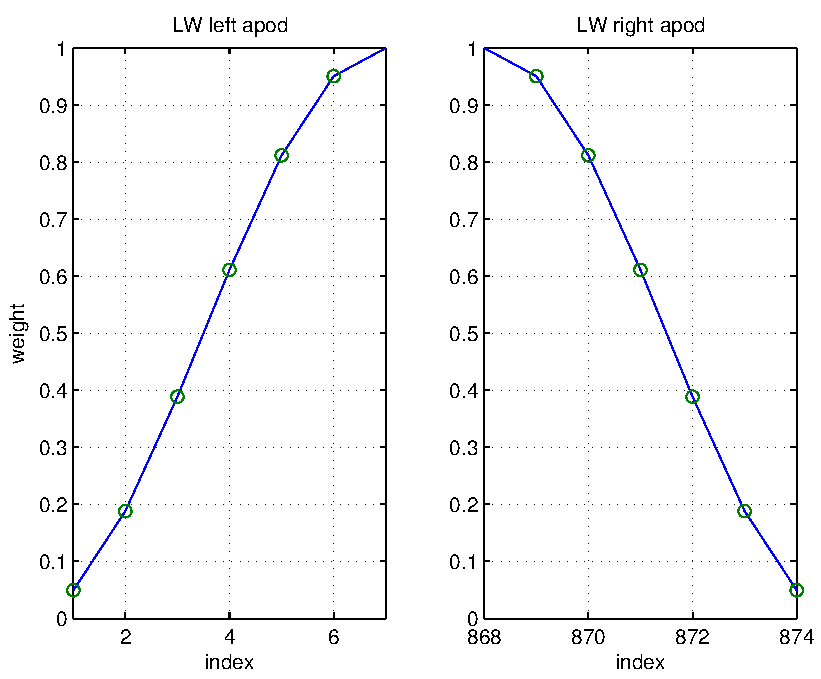
\includegraphics[scale=0.5]{figures/apod_LW.pdf}
\end{center}
edge of band details for the LW extended resolution apodization.
The apodization is symmetrical and all the weights are non-zero.
\end{frame}
%----------- slide --------------------------------------------------%
\begin{frame}
\frametitle{sweep direction differences}

\begin{itemize}

  \item as a proxy for sweep direction differences we compare 3-day
    means of FOR 15 and 16 for 8-10 Nov 2015

  \item for comparison purposes we include sweep direction
    differences for the {\ccast} and {\noaa} algorithms from the
    17-19 Feb 2015 tests

  \item the double differences shown here are \[(\mbox{\small FOR
    15} - \mbox{\small FOR 16}) - (\mbox{\small Hamming FOR 15} -
    \mbox{\small Hamming FOR 16})\]

  \item the Hamming apodization is applied to radiances before
    conversion to brightness temperatures, which in turn is done
    before taking means

\end{itemize}

\end{frame}
%----------- slide --------------------------------------------------%
\begin{frame}
\frametitle{ccast apodized extended resolution}
\begin{center}
  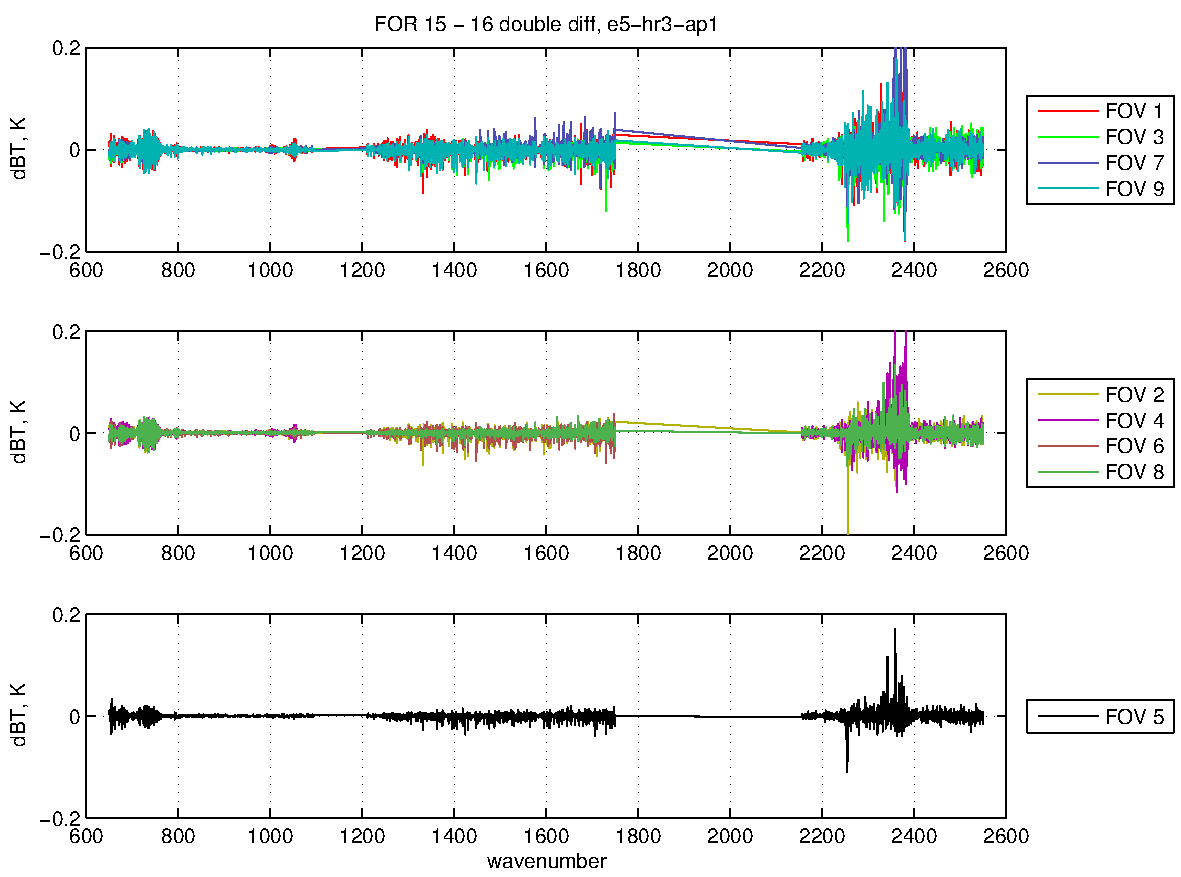
\includegraphics[scale=0.5]{figures/rel_ddif_e5_hr3_ap1.pdf}
\end{center}
\end{frame}
%----------- slide --------------------------------------------------%
\begin{frame}
\frametitle{ccast unapodized extended resolution}
\begin{center}
  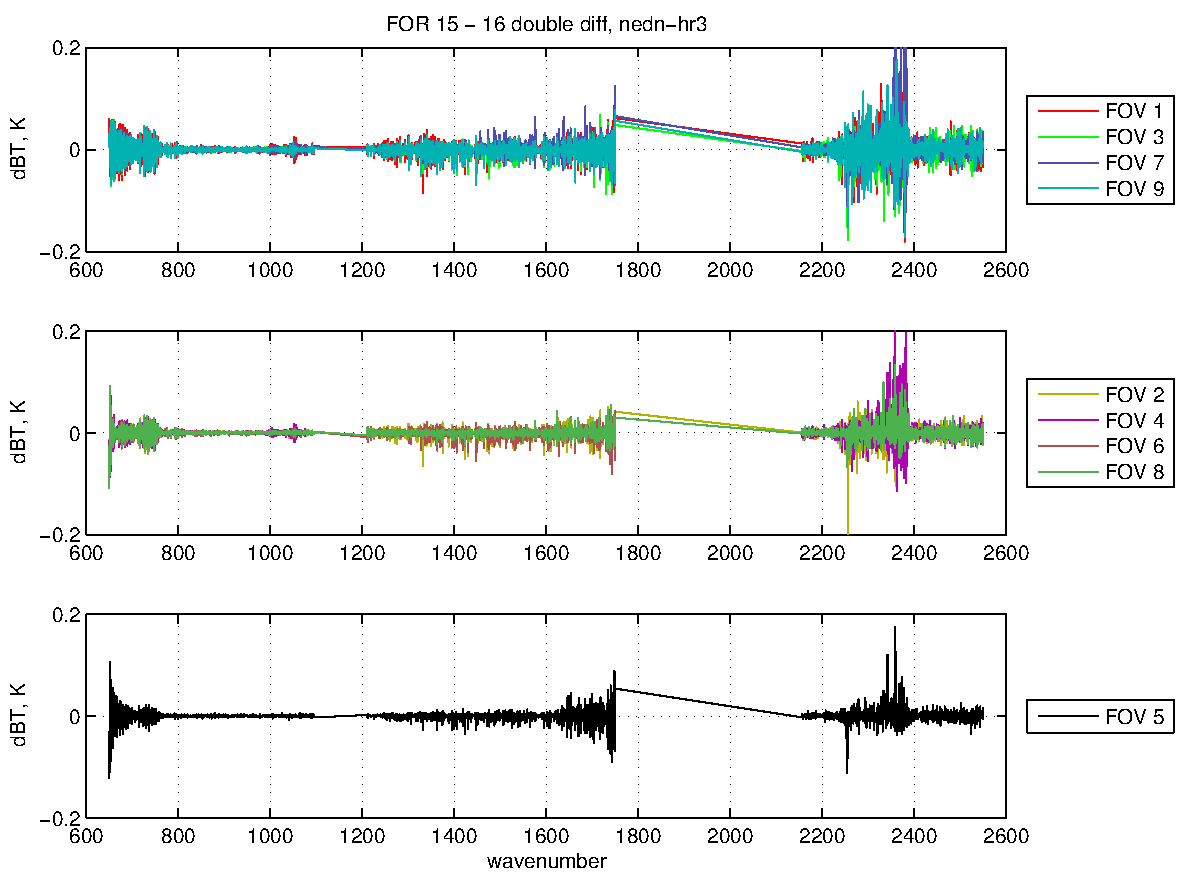
\includegraphics[scale=0.5]{figures/rel_ddif_e5_hr3.pdf}
\end{center}
\end{frame}
% %----------- slide --------------------------------------------------%
% \begin{frame}
% \frametitle{unapodized truncated resolution}
% \begin{center}
%   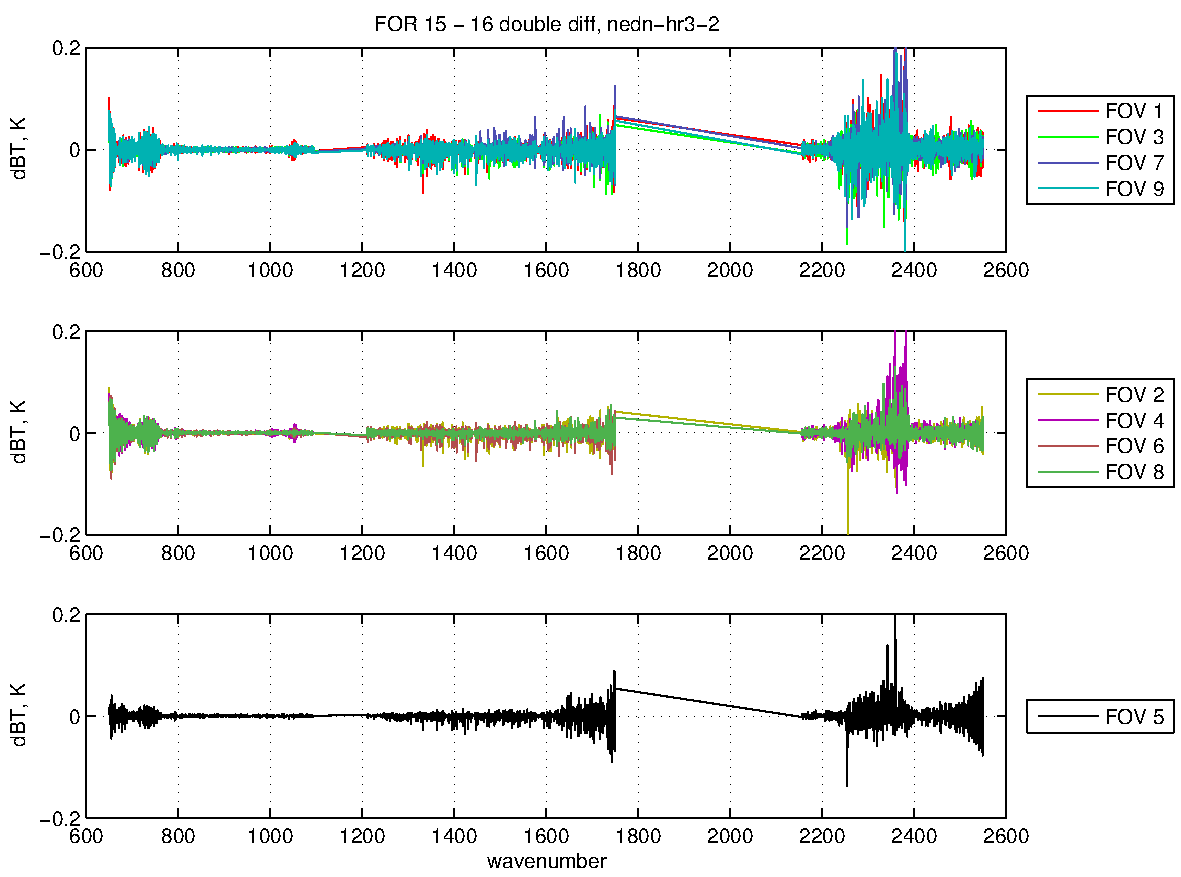
\includegraphics[scale=0.5]{figures/rel_ddif_e5_hr3-2.pdf}
% \end{center}
% \end{frame}
%----------- slide --------------------------------------------------%
\begin{frame}
\frametitle{noaa 17-19 feb 2015 high res tests}
\begin{center}
  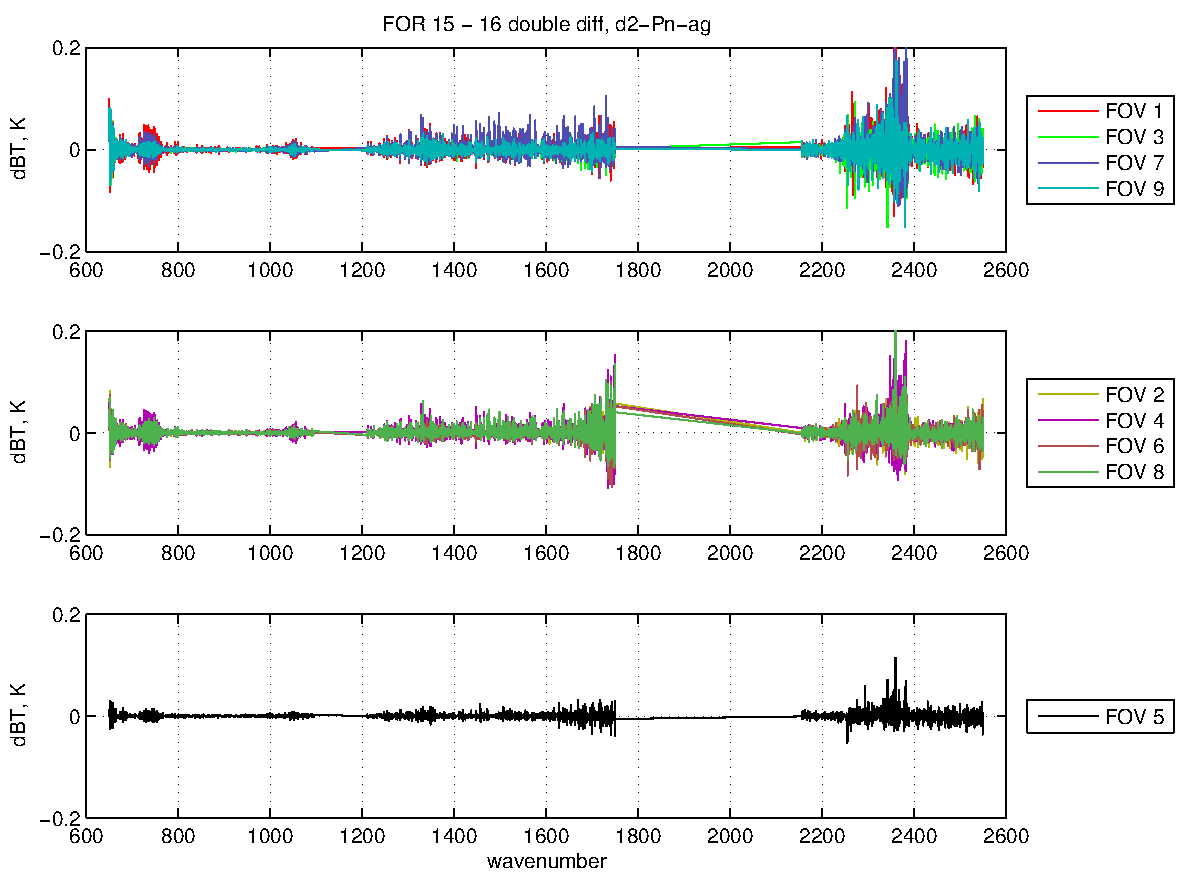
\includegraphics[scale=0.5]{figures/rel_noaa_ddif.pdf}
\end{center}
\end{frame}
%----------- slide --------------------------------------------------%
\begin{frame}
\frametitle{ccast 17-19 feb 2015 high res tests}
\begin{center}
  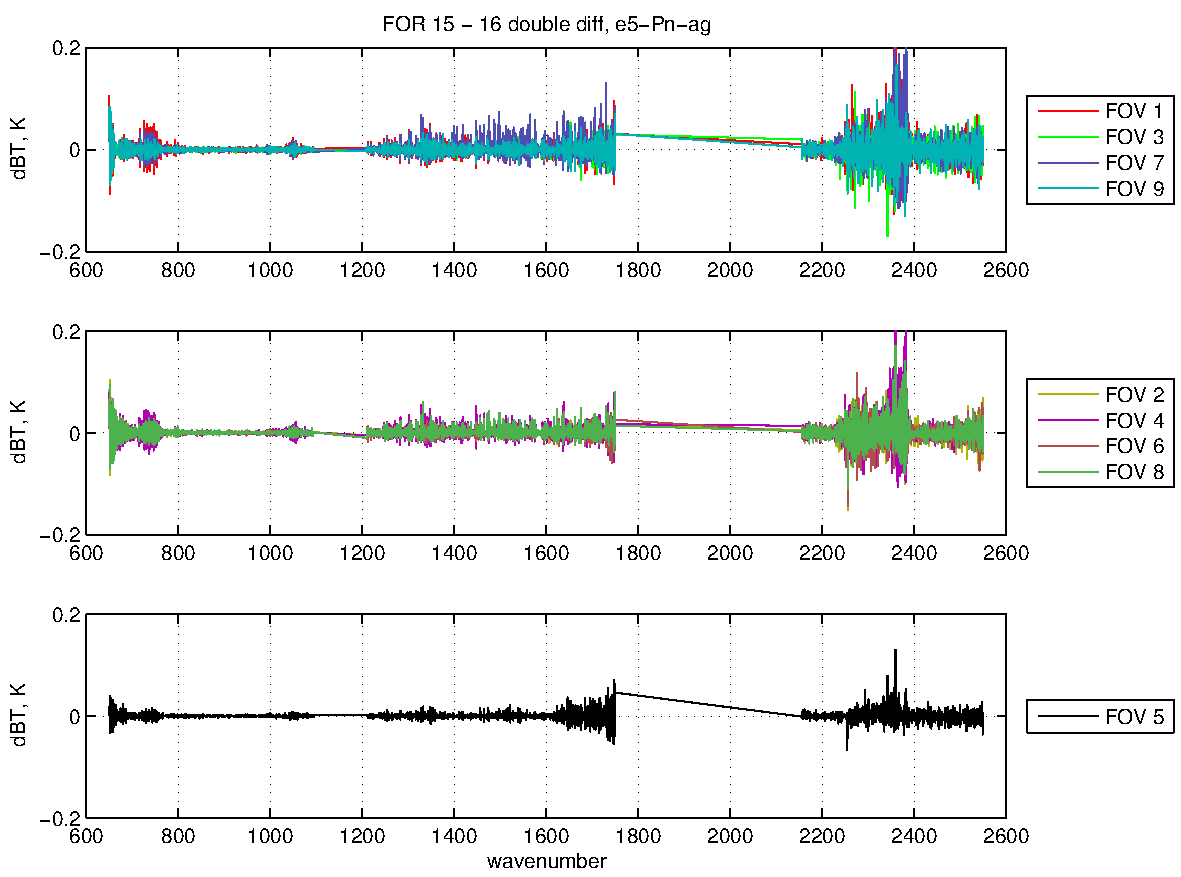
\includegraphics[scale=0.5]{figures/rel_ccast_ddif.pdf}
\end{center}
\end{frame}
%----------- slide --------------------------------------------------%
\begin{frame}
\frametitle{comments}

\begin{itemize}

  \item sweep direction differences are less with apodized extended
    resolution with the {\ccast} reference algorithm, in comparison
    with both {\ccast} without apodization and the best {\noaa} and
    {\ccast} results from the Feb 2015 tests

  \item these results would be more significant if we had included
    tests of apodized extended resolution using the {\noaa} reference
    algorithm.  (That should be easy but we forgot to update the
    point-dependent specs for the {\noaa} processing filters.)

  \item the following slide shows FOV 5 relative differences for the
    {\ccast} reference algorithm, with and without the extended
    apodization.  The apodization gives a significant improvement in
    the LW 

\end{itemize}

\end{frame}
%----------- slide --------------------------------------------------%
\begin{frame}
\frametitle{fov 5 relative differences}
\begin{center}
  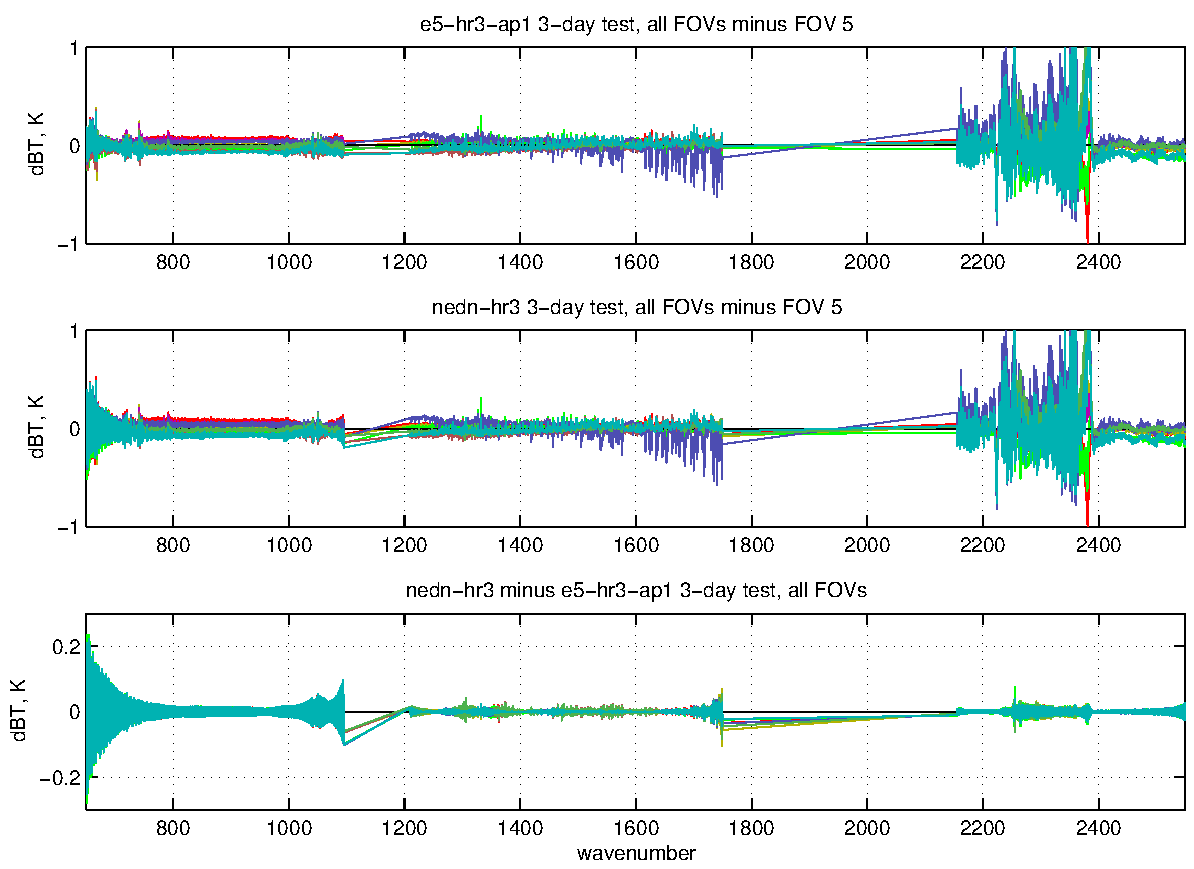
\includegraphics[scale=0.5]{figures/rel_summary.pdf}
\end{center}
\end{frame}
%----------- slide --------------------------------------------------%
\begin{frame}
\frametitle{conclusions}

\begin{itemize}

  \item applying a cosine apodization at the edges of the new
    extended interferograms reduces sweep direction and FOV 5
    relative residuals, in comparison to processing without such
    apodization

  \item further potential improvements such as circular shift should
    be compared with such an apodization rather than with standard
    processing

  \item with the apodization the FOV 7 nonlinearity dominates the
    FOV 5 relative residuals in the LW and MW

  \item several variations of the apodization shown here, including
    a 4-point symmetric function, a 7/6 point asymmetric function,
    and shifting all transforms to odd ($n-1$) point sets with the 6
    point function all gave similar or slightly worse results

\end{itemize}

\end{frame}
% %----------- slide --------------------------------------------------%
% \begin{frame}
% \frametitle{ccast calibration equation}
% 
% \[\rES = F \cdot \rIT \cdot f \cdot \SA^{-1}\cdot f \cdot 
%          \frac{\ES - \SPmean}{\ITmean - \SPmean} \]
% 
% \begin{itemize}
%   \item $\rES$ is calibrated earth-scene radiance at the user grid
%   \item $F$ is Fourier interpolation from sensor to user grid
%   \item $\rIT$ is expected ICT radiance at the sensor grid
%   \item $f$ is a raised-cosine bandpass filter with wings at or just
%     inside instrument responsivity
%   \item $\SA$ is from a periodic sinc ILS wrapping at the sensor
%     grid
%   \item $\ES$, $\ITmean$ and $\SPmean$ are corrected for
%     nonlinearity
%   \item $\ITmean$ and $\SPmean$ are averages over 9 scans
% \end{itemize}
% 
% \end{frame}
%----------- slide --------------------------------------------------%
\end{document}

